This sections evaluates the performance of proposed methodology in estimating correspondences of human poses in-the-wild. Results for quantitative an qualitative experiments are reported. Experiments \ref{exp:internal} investigate the accuracy of estimating dense correspondences of non-rigid deformable objects, and the impact of annotating outlines of human poses instead of annotating skeletons. Experiments \ref{exp:benchmark} compare the joints localisation accuracy of our skeleton prediction from outline fitting with respect to that of state-of-the-art human pose estimation algorithms in-the-wild. Note that all results reported in this section were obtained by fitting Patch AAM using the fast version of the Simultaneous Inverse Compositional algorithm (Fast-SIC) originally proposed by the authors of \cite{Papandreou2008}. For further experimental results and visualisations please refer to our supplementary material. 

\subsection{Databases \& Error Metrics}

\subsection{Internal Evaluation}
\label{exp:internal}

\begin{figure}[t!]
    \centering
    \begin{subfigure}[b]{0.23\textwidth}
            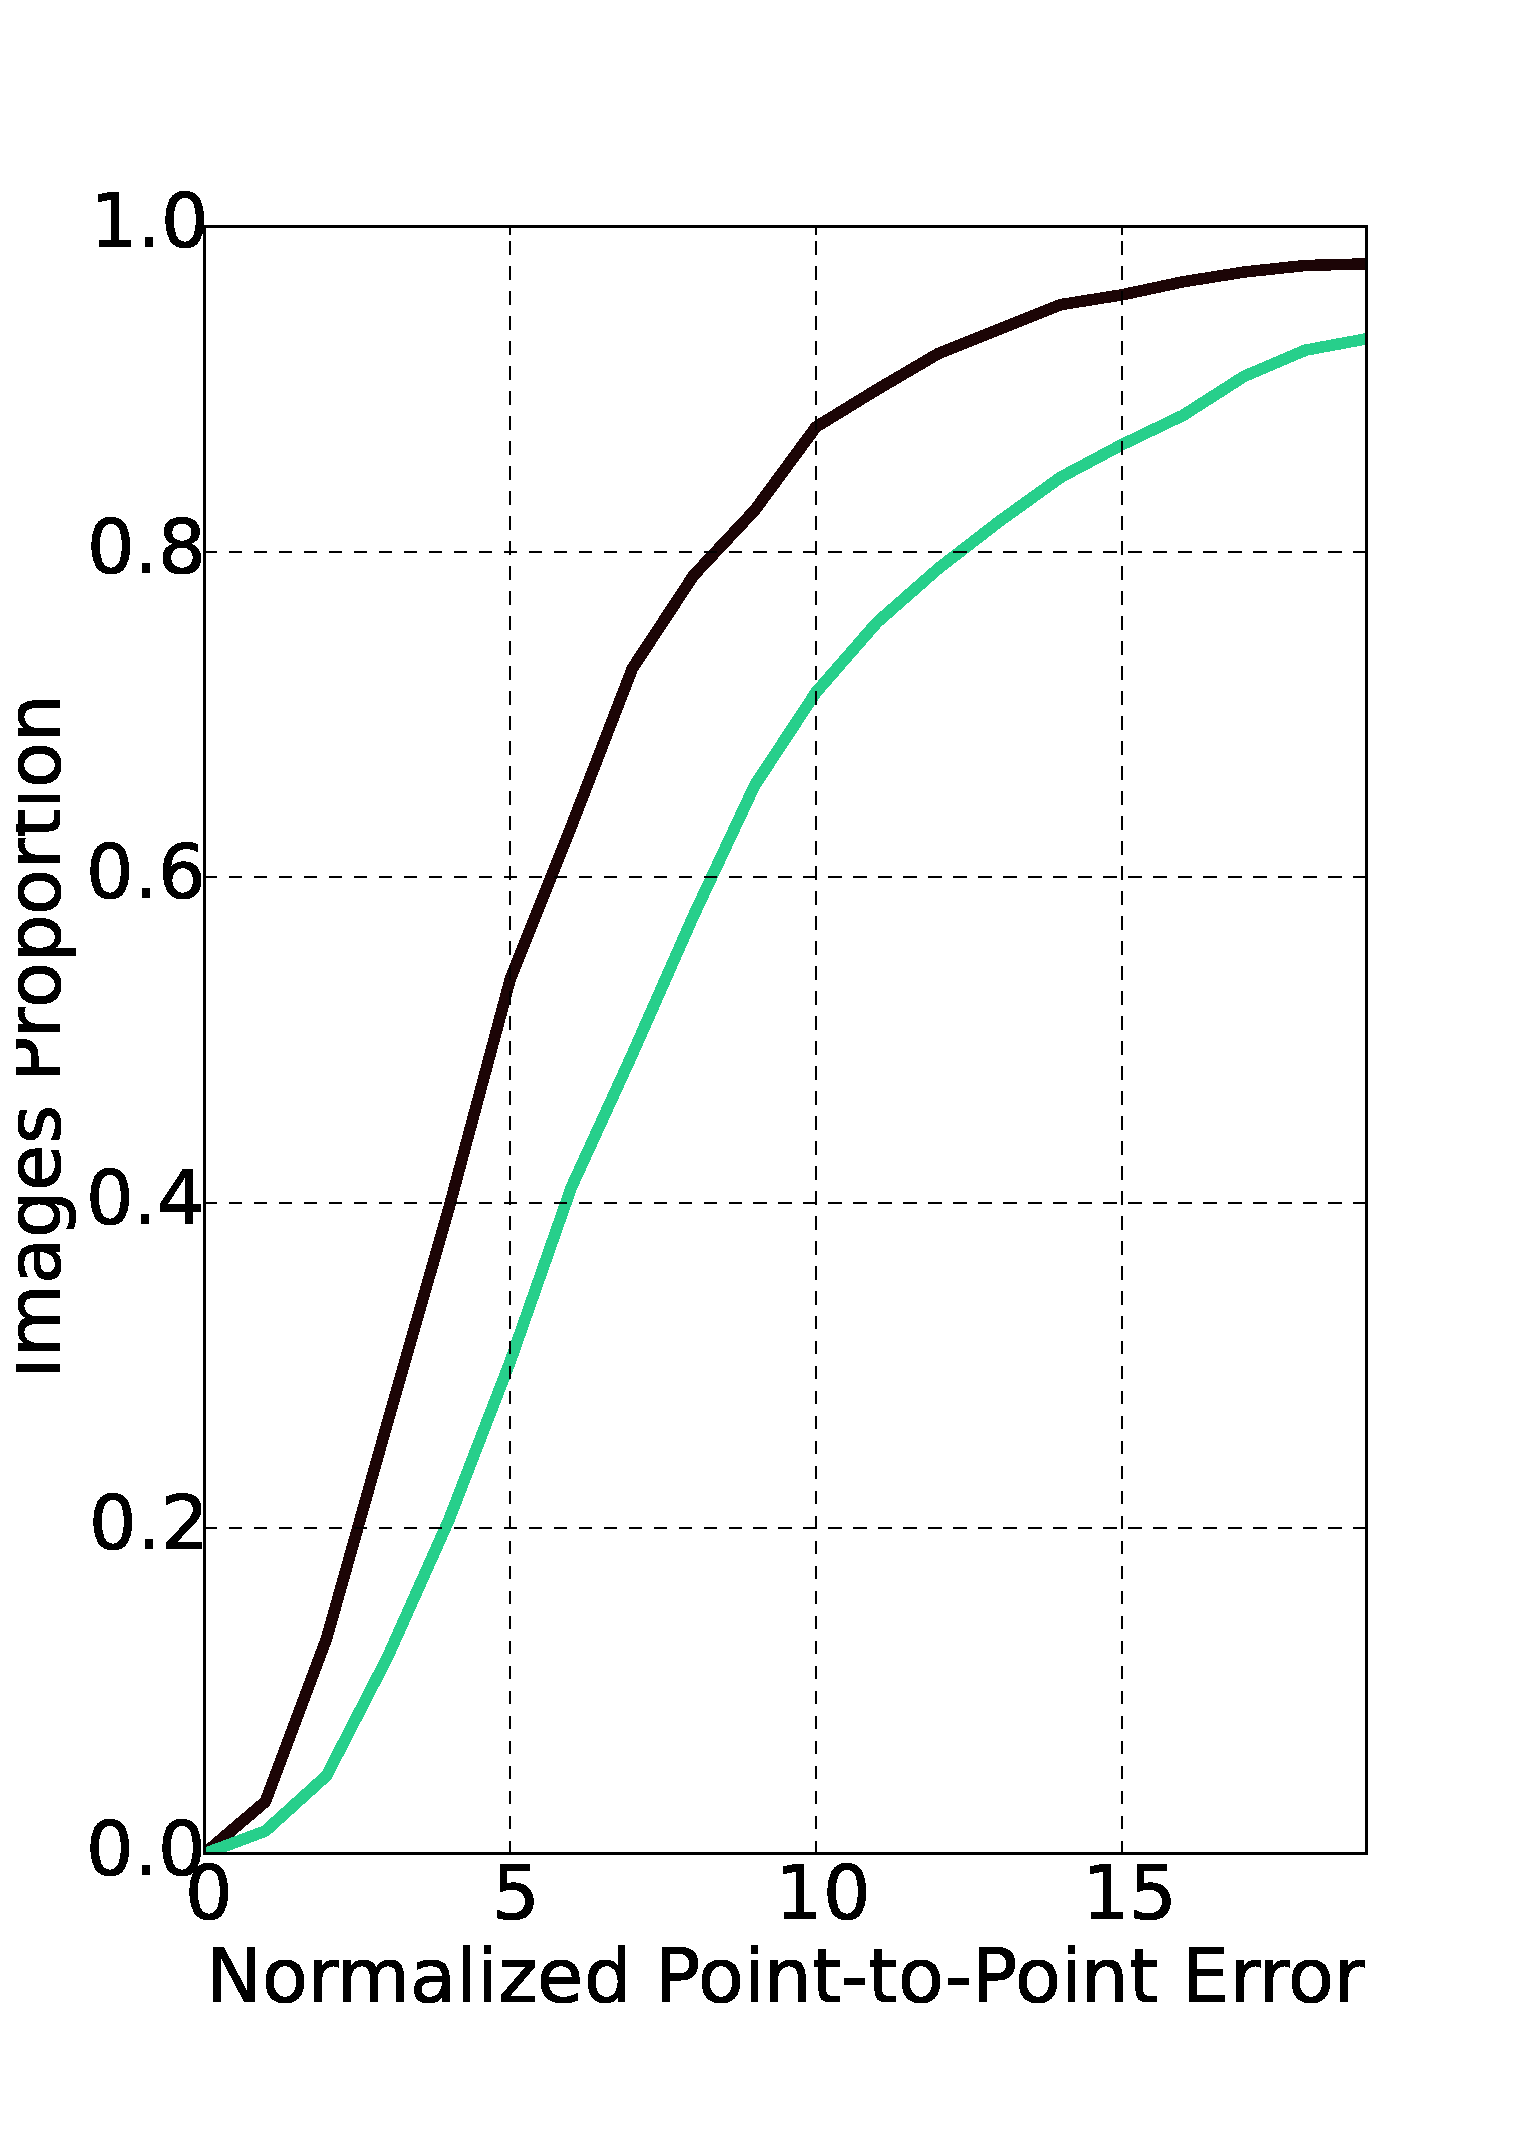
\includegraphics[width=\textwidth]{resources/HandBenchmark/elbow_joints}
    \end{subfigure}
    \hfill
    \begin{subfigure}[b]{0.23\textwidth}
            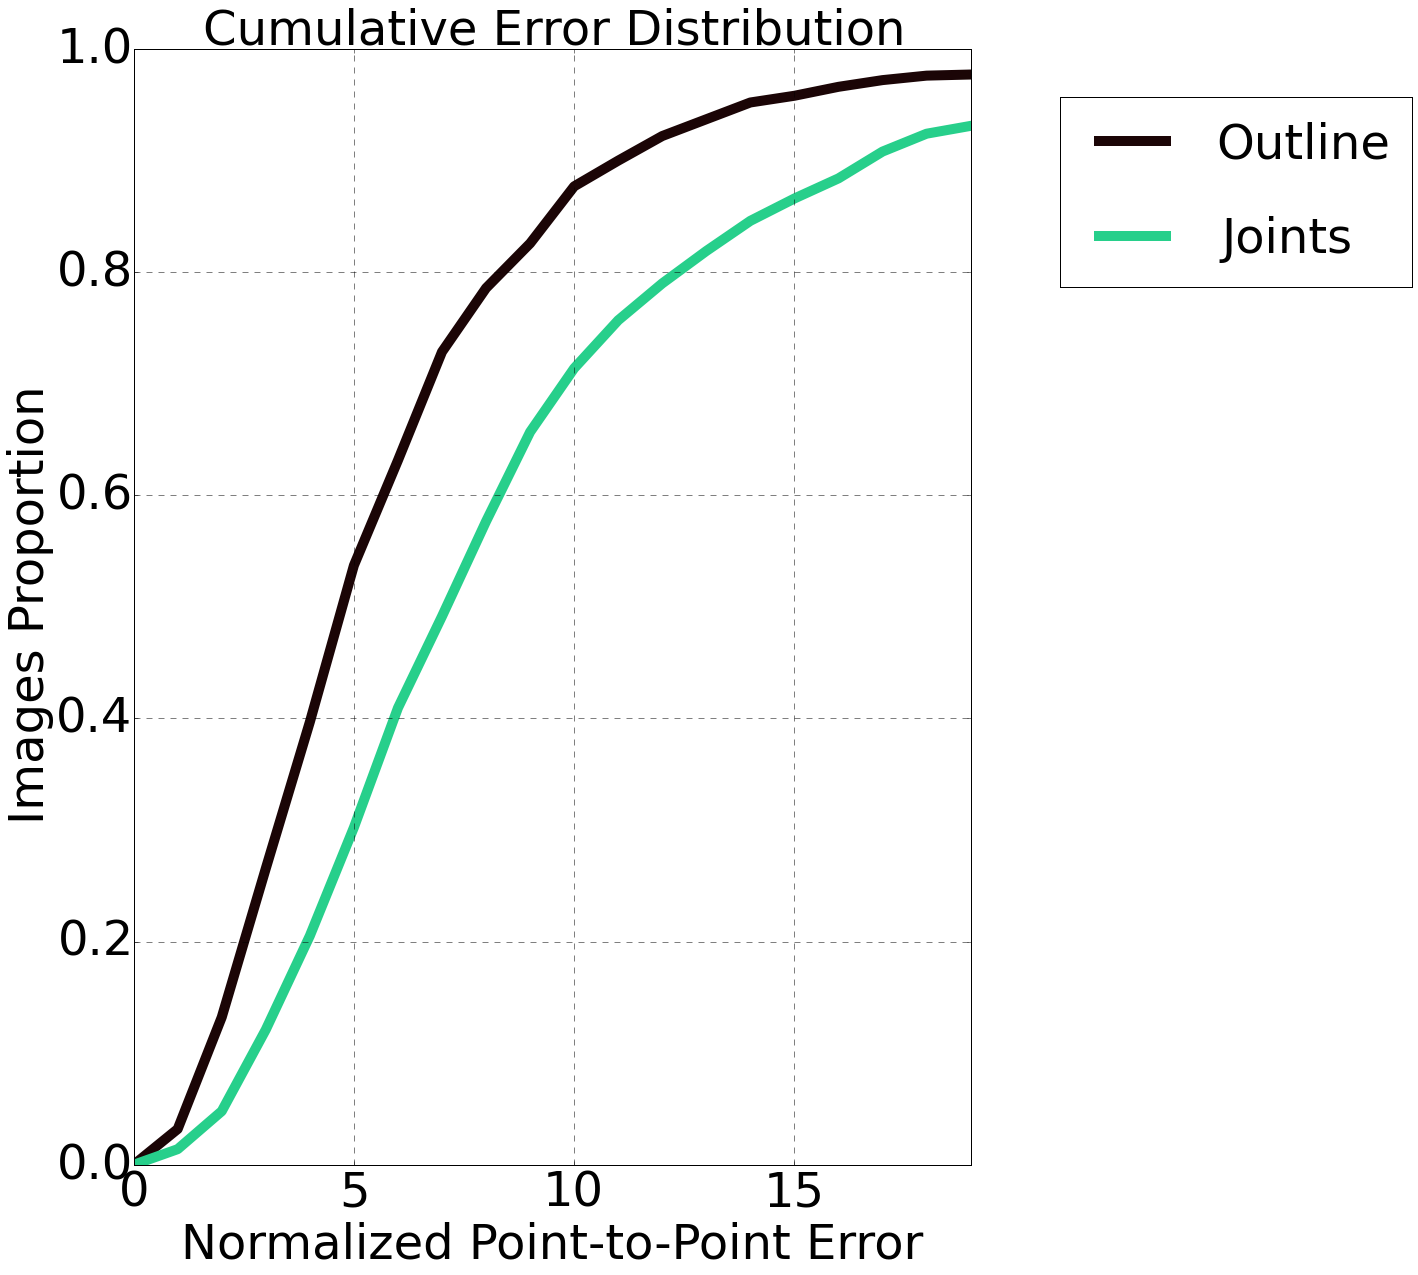
\includegraphics[width=\textwidth]{resources/HandBenchmark/wrist_joints}
    \end{subfigure}
    \caption{Hand Benchmark.}
    \label{fig:internal_benchmark}
\end{figure}

\subsection{Benchmark Against State-if-the-art}
\label{exp:benchmark}

\begin{figure}[t!]
    \centering
    \begin{subfigure}[b]{0.23\textwidth}
            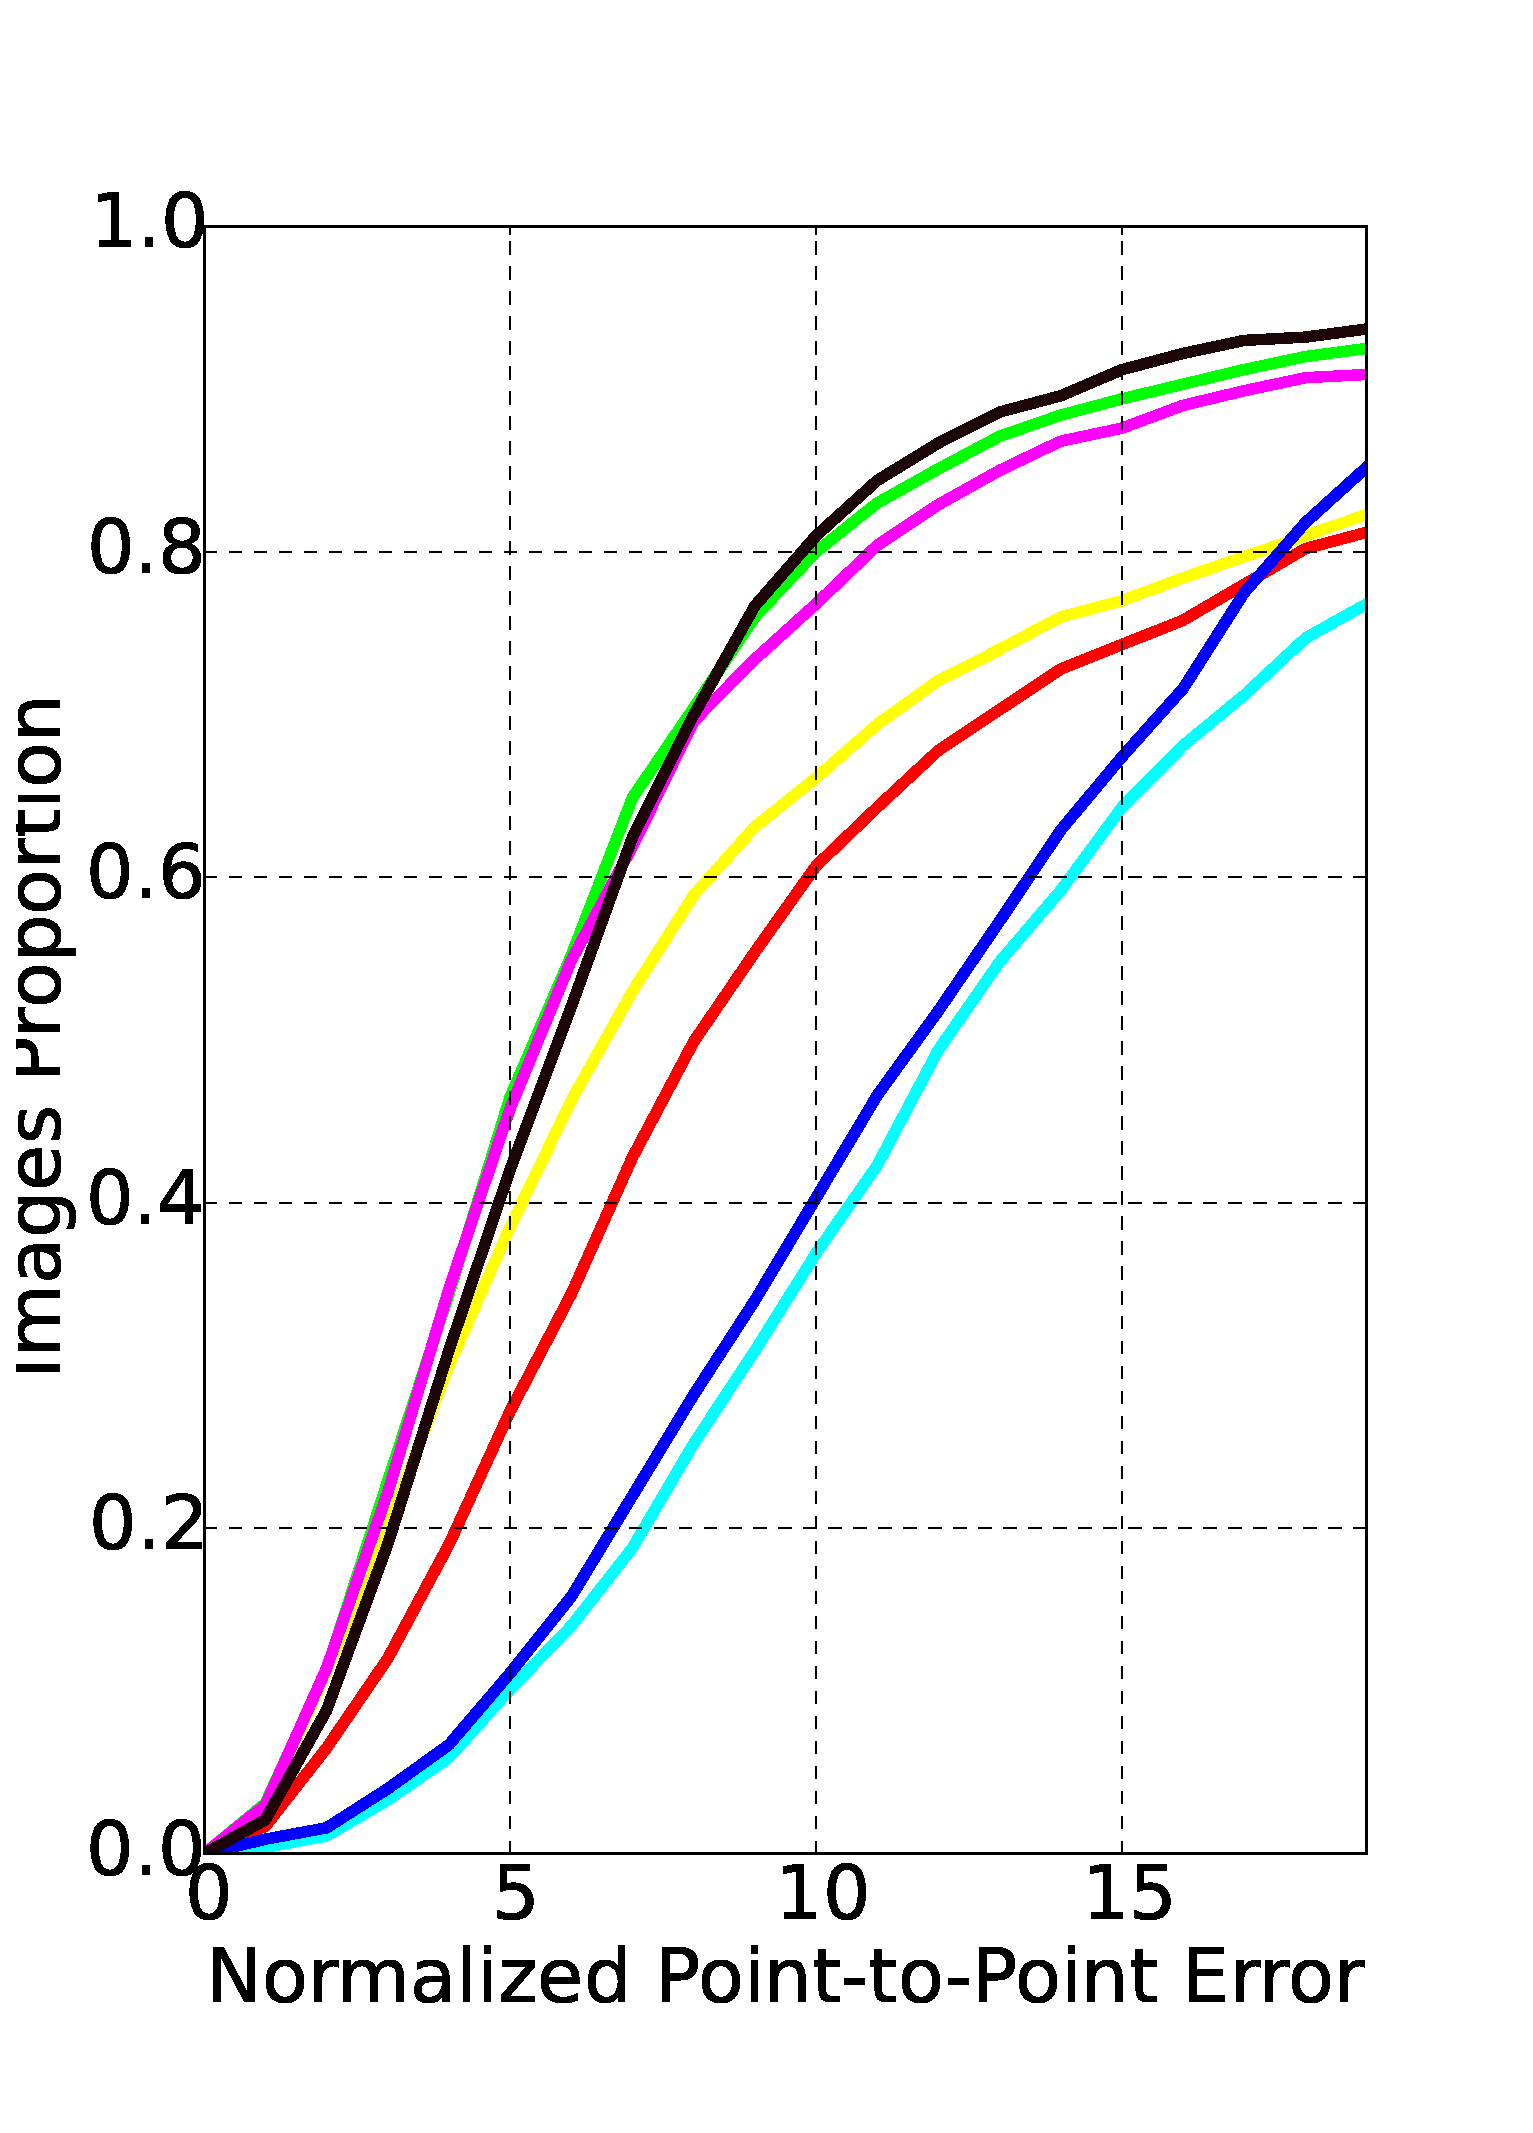
\includegraphics[width=\textwidth]{resources/HandBenchmark/elbow}
    \end{subfigure}
    \hfill
    \begin{subfigure}[b]{0.23\textwidth}
            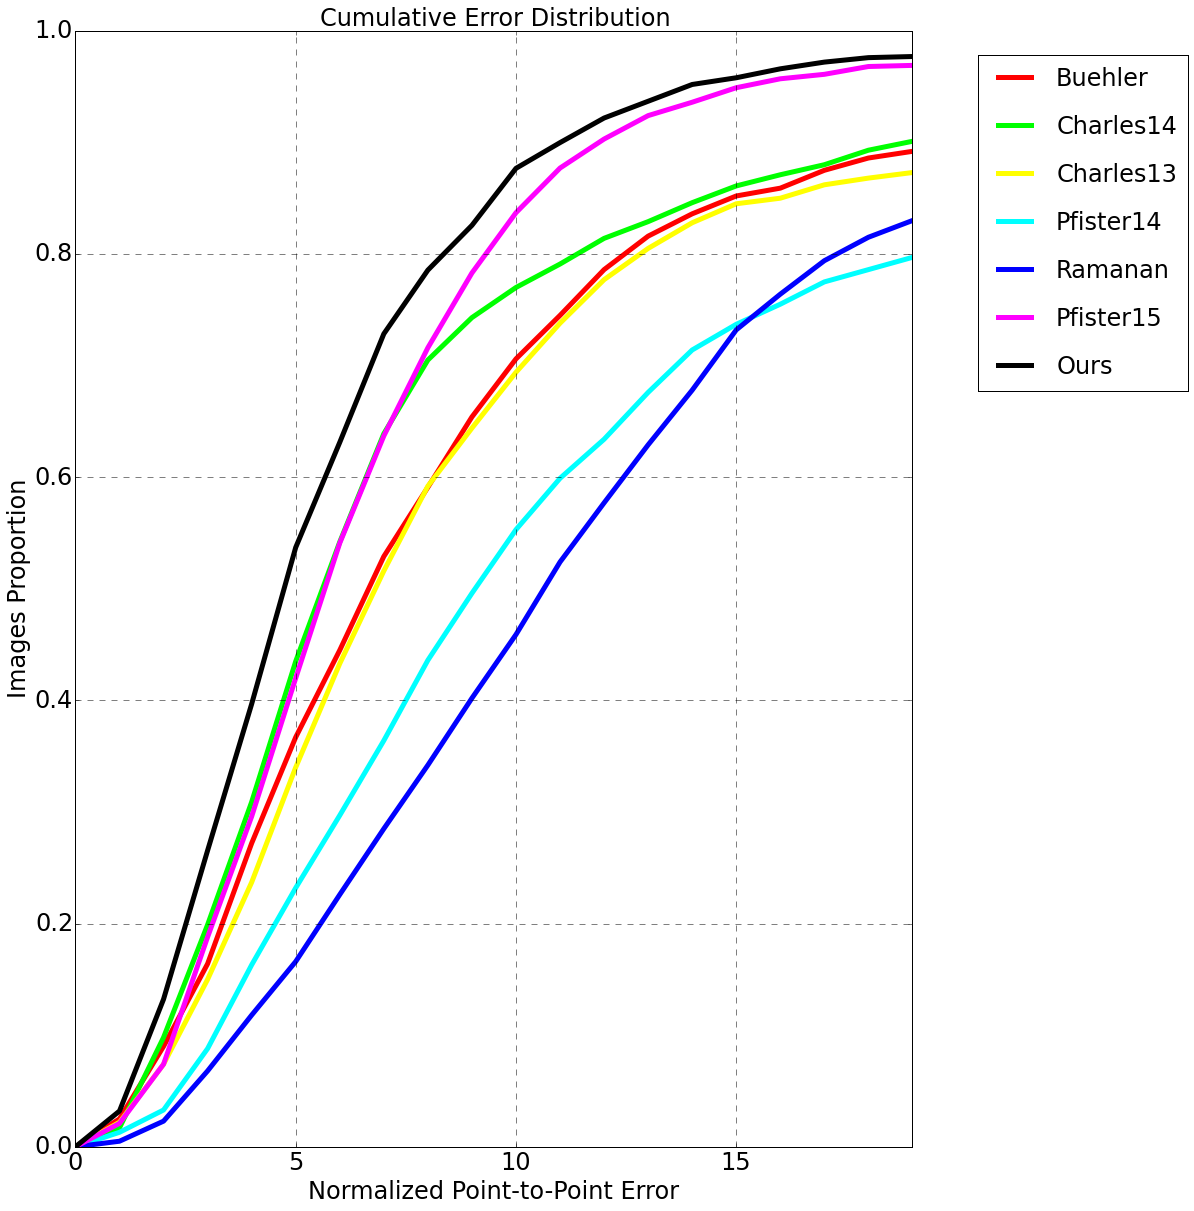
\includegraphics[width=\textwidth]{resources/HandBenchmark/wrist}
    \end{subfigure}
    \caption{Hand Benchmark.}
    \label{fig:hand_benchmark}
\end{figure}


\subsection{Qualitative Results}
\label{exp:qualitative}

